% !TeX spellcheck = id_ID
\documentclass[a4paper,12pt]{article}
\usepackage[bahasa]{babel}
\usepackage{graphicx}
\usepackage{multirow}
\usepackage{enumitem}
\usepackage[T1]{fontenc}
\usepackage{inconsolata}
\usepackage{lipsum}
\usepackage{xcolor}

\graphicspath{ {./img/} }
\begin{document}
\title{ {\Large Laporan Praktikum}\\ Jaringan Komputer \\{\Large Pertemuan 10}}

\author{Aldzikri Dwijayanto Prathama 
	\\195410189
	\\Teknik Informatika}
\makeatletter
\begin{titlepage}
	\begin{center}
		{\huge \bfseries \@title }\\[14ex]
		
\includegraphics[scale=.8]{logo}\\[4ex]
		{\large \@author}\\[19ex]
		{\large \bfseries {SEKOLAH TINGGI MANAJEMEN INFORMATIKA DAN KOMPUTER
				AKAKOM YOGYAKARTA}}
	\end{center}


{\large \@date} 
\end{titlepage}
\makeatother
\newpage
\tableofcontents
\newpage

\section{Tujuan}
Mahasiswa mampu melakukan konfigurasi NAT untuk mengakses Internet

\section{Dasar Teori}
Penafsiran alamat jaringan (Network Address Translation atau NAT) adalah suatu
metode untuk menghubungkan lebih dari satu komputer ke jaringan Internet dengan
menggunakan satu alamat IP. Banyaknya penggunaan metode ini disebabkan karena
ketersediaan alamat IP yang terbatas, kebutuhhan akan keamanan (security), dan
kemudahan serta fleksibilitas dalam administrasi jaringan.

\begin{center}
	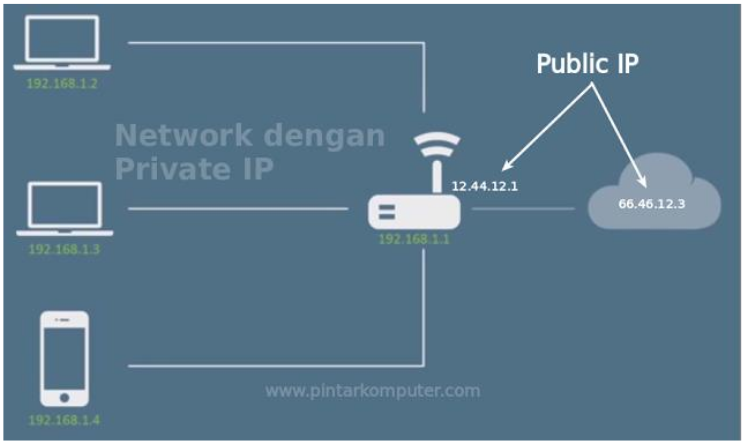
\includegraphics[scale=.3]{dasar}
\end{center}

\paragraph{Alamat IP yang terbatas\\}
Saat ini, IPv4 masih banyak digunakan. Oleh karena IPv4 menggunakan 32 bit,
maka secara teoritis hanya terdapat 2 32 alamat = 4.294.967.296 alamat IP saja. Karena
keterbatasan inilah sebagian besari ISP (Internet Service Provider) hanya akan
mengalokasikan satu alamat untuk satu pengguna dan alamat ini bersifat dinamik, artinya
alamat IP yang diberikan akan berbeda setiap kali user melakukan koneksi ke Internet,
akan tetapi juga hanya tersedia satu IP untuk satu komputer saja yang dapat terkoneksi
ke Internet. Hal ini dapat diatasi dengan menggunakan NAT. Dengan NAT gateway yang
dijalankan pada salah satu komputer, satu alamat tersebut dapat dibagi ke komputer lain
sehingga semuanya dapat terkoneksi ke Internet secara bersamaan.

\paragraph{Keamanan\\}
Ketika sebuah komputer terkoneksi ke Internet, komputer tersebut tidak hanya
terkoneksi ke salah satu server suatu situs tertentu, namun sangat mungkin juga diakses
oleh komputer lain yang juga terkoneksi ke Internet. Jika disalahgunakan, tentunya sangat
berbahaya. Data-data penting dapat dilihat dan dicuri oleh pihak lain. NAT secara otomatis
memberikan proteksi seperti halnya firewall dengan hanya mengijinkan koneksi yang
berada di dalam jaringan LAN.

\paragraph{Administrasi Jaringan\\}
Dengan NAT, suatu jaringan yang besar dapat dipecah-pecah menjadi jaringan-
jaringan yang lebih kecil. Bagian-bagian kecil tersebut memiliki satu alamat IP, sehingga
dapat menambahkan atau mengurangi jumlah komputer tanpa mempengaruhi jaringan
secara keseluruhan. Selain itu, pada gateway NAT modern terdapat server DHCP yangdapat mengkonfigurasi komputer client secara otomatis. Selain itu, gateway NAT dapat
membatasi akses ke Internet, juga mampu mencatat semua lalu lintas data, dari dan ke
Internet. Secara keseluruhan, dengan segala kelebihan gateway NAT tersebut, admin
jaringan akan sangat terbantu dalam melakukan tugas-tugasnya.

\section{Praktik}
\begin{enumerate}
	\item \textbf{Instalasi Jaringan}\\
	Langkah pertama adalah menyambungkan router dengan jaringan, port ether1 yang berperan sebagai dhcp client disambungkan ke jaringan internet akakom, lalu ether2 disambungkan ke pc1, sedangkan ether3 yang akan memiliki dhcp server disambungkan ke pc2. 
	
	\item \textbf{Menghapus konfigurasi Mikrotik}\\
	\begin{center}
		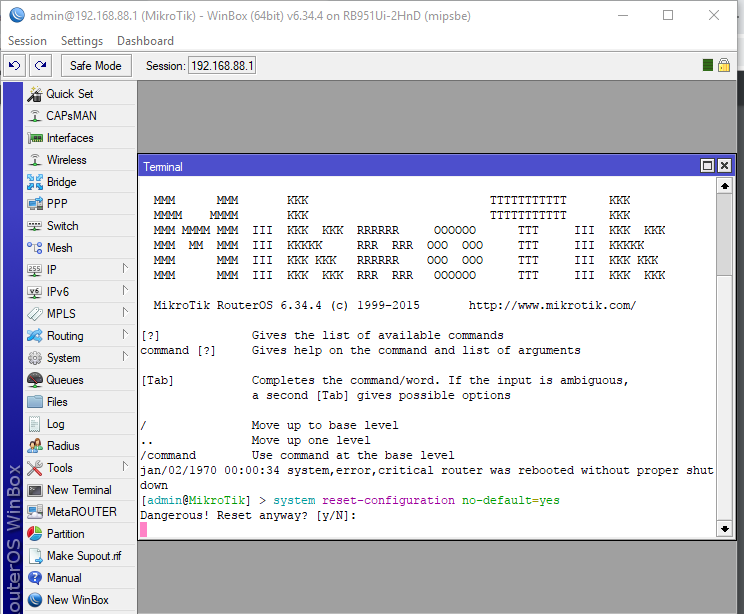
\includegraphics[scale=.4]{Capture1}
	\end{center}
	Untuk me-reset konfigurasi pada mikrotik, pertama login terlebih dahulu dengan winbox, lalu kilk new terminal dan tuliskan \texttt{system reset-configuration no-default=yes}, perintah tersebut akan mereset router tanpa konfigurasi default. Lalu tekan y untuk konfirmasi.Maka Mikrotik akan booting dan konfigurasinya telah dihapus semua. Lalu login kembali dengan mac address.
	
	\item \textbf{Cek IP Address pada Interface.\\}
	Klik menu IP → Addresses, maka akan muncul kotak windows Address List dan
	pastikan pada kotak tersebut masih kosong.
	\begin{center}
		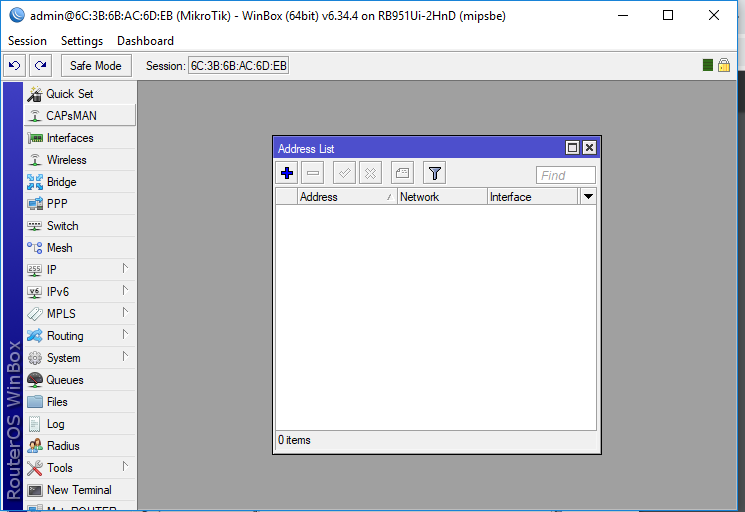
\includegraphics[scale=.5]{Capture2}
	\end{center}
	
	\item \textbf{Setting DHCP Client pada Ether 1.\\}
	klik IP lalu pilih dhcp client, maka muncul jendela dhcp, kemudian klik "+", maka muncul jendela New DHCP Client.
	\begin{center}
		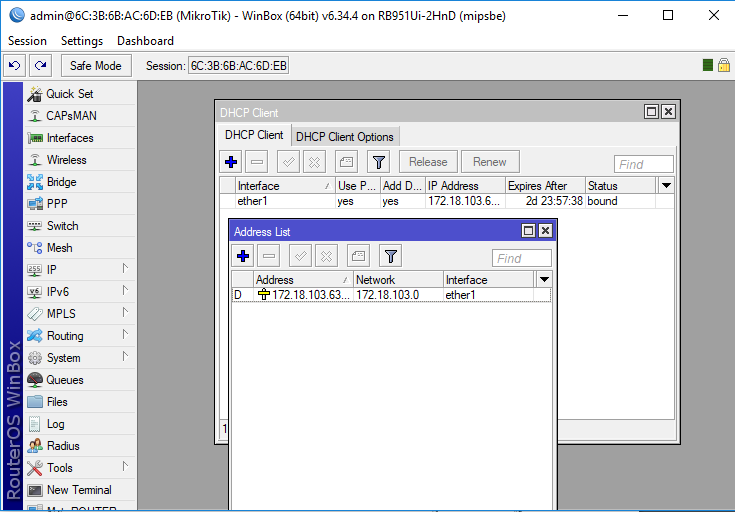
\includegraphics[scale=.5]{Capture5}
	\end{center}
	 Pada tab DHCP, pilih Interface-nya: Ether1 (dengan cara klik tombol panah bawah
	, lalu klik Ether1), lalu klik tombol Apply. Langkah berikutnya klik tab Status, untuk melihat IP Address, Gateway, DHCP
	Server, Primary DNS, dll. yang didapat DHCP Client di Ether1 dari DHCP Server
	yang ada di laboratorium, seperti pada Gambar berikut: (alamat IP Address yang
	di dapat berbeda-beda). Lalu klik tombol OK, dan pastikan pada kotak windows DHCP Client terdapat interface
	Ether1 yang telah di konfigurasi sebagai DHCP Client dan pastikan juga pada kotak
	windows Address List, Ether1 telah mendapat IP yang sama dengan yang ada pada
	kotak windows DHCP Client.Sampai dengan langkah ini, berarti Ether1 telah mendapatkan IP yang disewakan oleh
	DHCP Server yang berada di laboratorium.
	
	\item \textbf{Menambahkan IP Address pada Ether2.\\}
	Klik menu IP → Addresses, maka akan muncul kotak windows Address List.
	\begin{center}
		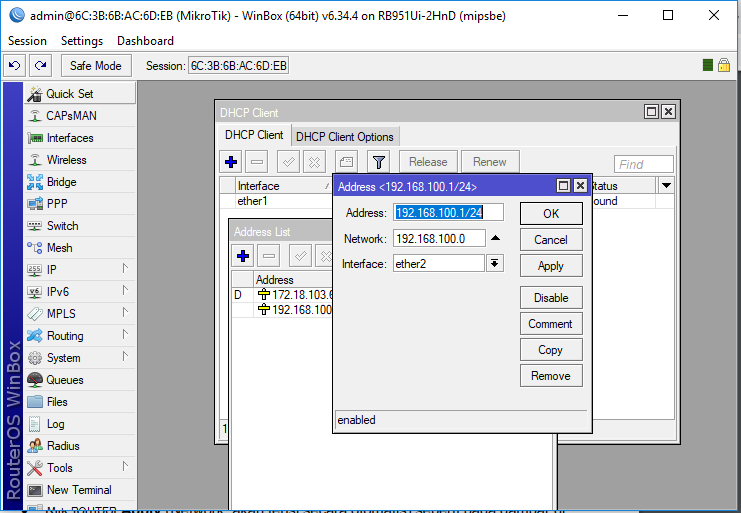
\includegraphics[scale=.5]{Capture6}
	\end{center}
	Lalu klik tombol "+", maka muncul window New address Isikan alamat IP pada Address: 192.168.168.100.1/24 dan Interface: Ether2. Klik tombol Apply (Network, akan terisi secara otomatis) seperti pada gambar di
	bawah ini.Lalu klik tombol OK, sampai dengan langkah ini, berarti Ether2 memiliki IP yang diisikan dan dapat dilihat pada kotak windows Address List (termasuk Ether1).
	
	\item \textbf{Menambahkan IP Address pada Ether3\\}
	Klik menu IP → Addresses, maka akan muncul kotak windows Address List. Lalu klik tombol "+"
	, maka akan muncul kotak window New Address,
	i sikan alamat IP pada Address: 172.18.10.1/24 dan Interface: Ether3, lalu klik
	tombol Apply (Network, akan terisi secara otomatis) seperti pada gambar di
	bawah ini. Lalu klik tombol OK, sampai dengan langkah ini, berarti Ether3 memiliki IP yang
	diisikan dan dapat dilihat pada kotak windows Address List (termasuk Ether1 dan
	Ether2).
	\begin{center}
		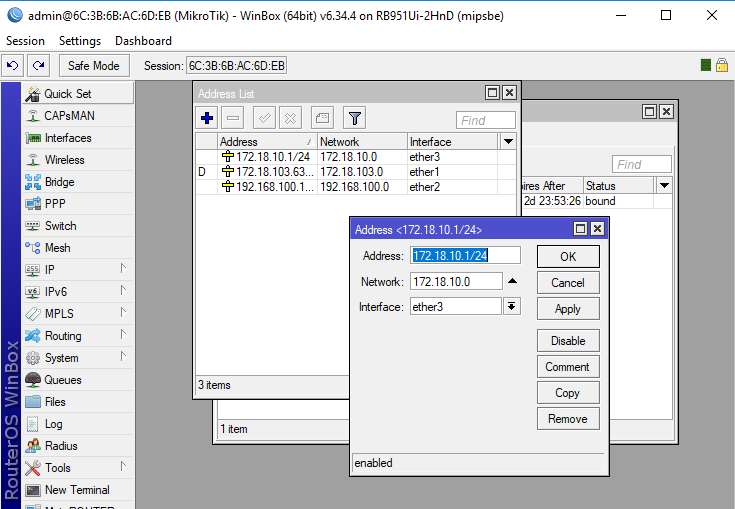
\includegraphics[scale=.5]{Capture7}
	\end{center}
	
	\item\textbf{Setting IP address pada komputer yang terhubung ke Ether2}\\
	Klik kanan pada icon Network , kemudian akan muncul 2 menu dan pilih menu
	Open Network \& Internet settings.
	\begin{center}
		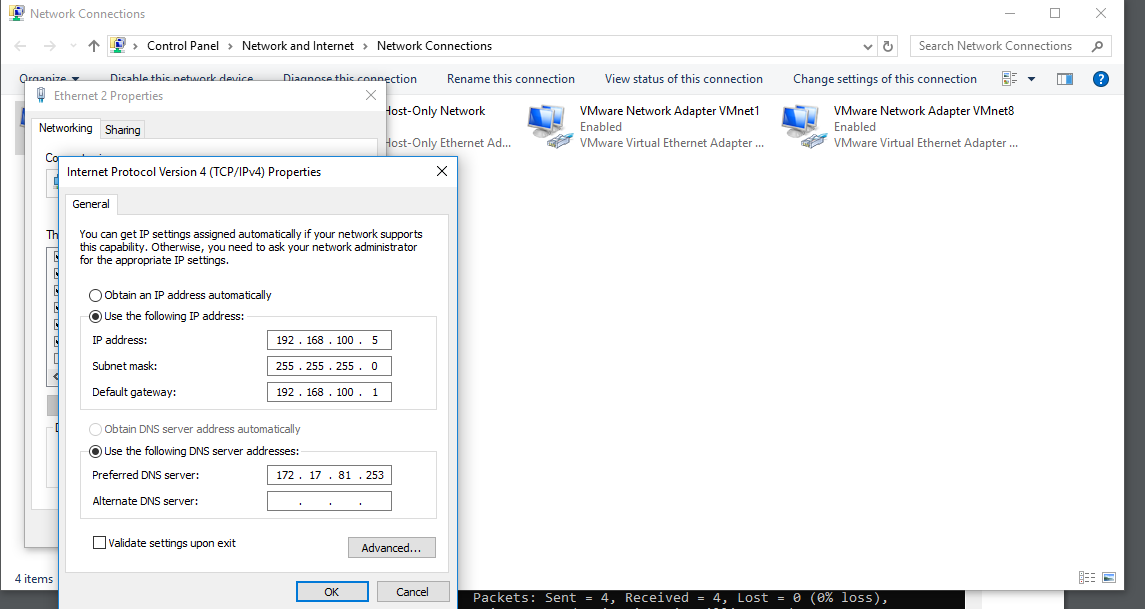
\includegraphics[scale=.5]{Capture8}
	\end{center}
	Akan muncul kotak window Setting, pilih menu Change adapter option.
	Tampil kotak window Network Connections, klik kanan Ethernet (yang mau diberikan IP Address), lalu pilih menu Properties. Maka akan tampil kotak window Ethernet Properties, double klik Internet Protocol Version 4 (TCP/IPv4), lalu pilih Use the following IP address, isi IP address: 192.168.100.5, Subnet mask: 255.255.255.0 Default gateway:
	192.168.100.1 dan Preferred DNS server: 172.17.81.253 (sesuai dengan alamat IP pada Primary DNS di Ether1, pada waktu konfigurasi DHCP Client).
	Kemudian klik tombol OK, dan lakukan tes koneksi dengan perintah Ping ke Gateway-nya: 192.168.100.1 dan pastikan terkoneksi.
	\begin{center}
		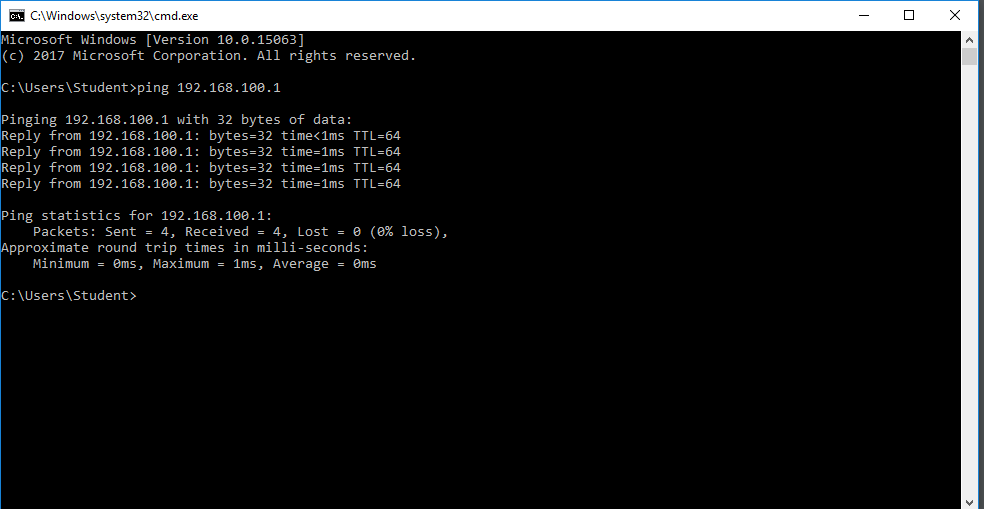
\includegraphics[scale=.4]{Capture9}
	\end{center}
	
	\item \textbf{Setting DHCP Server pada Interface Ether3}\\
	\begin{center}
		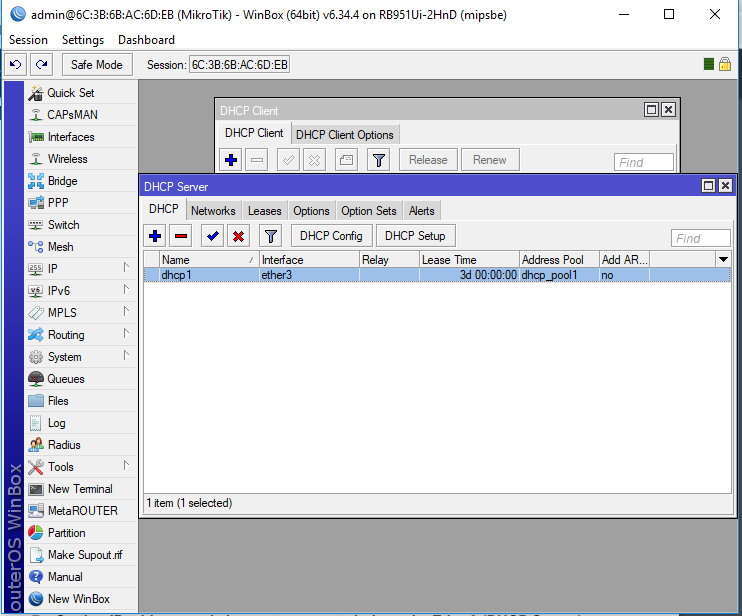
\includegraphics[scale=.5]{Capture10}
	\end{center}
	Pilih menu IP → DHCP Server, akan muncul kotak window DHCP Server, lalu klik menu DHCP Setup.
	Akan muncul kotak window DHCP Setup, lalu pada isian DHCP Server Interface
	
	pilih interface: Ether3 dengan cara klik tombol panah bawah terlebih dahulu. Klik tombol Next, pada isian DHCP Address Space alamat network dan netmasknya: 172.18.10.0/24 (secara otomatis berdasarkan setting IP Address pada interface Ether3).
	Klik tombol Next, pada isian Gateway for DHCP Network: 172.18.10.1 yang akan dijadikan sebagai gateway untuk setiap DHCP Client-nya (secara otomatis sama dengan IP Address pada interface Ether3).
	Klik tombol Next, pada isian Addresses to Give out: 172.18.10.2 – 172.18.10.254 (merupakan range IP Address yang akan diberikan (tepatnya disewakan) ke setiap DHCP Client-nya. (pada praktik kali ini silahkankan di ubah range-nya dari 172.18.10.2 – 172.18.10.10 sehingga komputer client akan menerima IP Address sesuai range tersebut.
	Klik tombol Next, pada isian DNS Server: 172.17.81.253 (akan berisi alamat DNS Server yang telah didapat mikrotik, dapat dilihat pada menu IP → DNS), dapat diganti dengan alamat DNS Server yang lain.
	Klik tombol Next, pada isian Lease Time: 3d 00:00:00 (akan berisi lama waktu IP Address dipinjamkan ke Client), isian ini berarti dipinjamkan selama 3 hari. Untuk menghindari penuh atau kehabisan IP, setting Lease-Time jangan terlalu lama, misalkan 1 hari saja.
	Klik tombol Next, maka akan tertampil pesan yang menyatakan bahwa setting DHCP telah berhasil.
	
	\item \textbf{Setting IP address pada komputer yang terhubung ke Ether3 (DHCP Server)}\\
	Klik kanan pada icon Network , kemudian akan muncul 2 menu dan pilih menu
Open Network \& Internet settings. Akan muncul kotak window Setting, pilih menu Change adapter option.
	Tampil kotak window Network Connections, klik kanan Ethernet (yang mau diberikan IP Address), lalu pilih menu Properties.
	Maka akan tampil kotak window Ethernet Properties, double klik Internet Protocol Version 4 (TCP/IPv4), lalu pilih Obtain an IP address automatically dan Obtain DNS server address automatically.Kemudian klik tombol OK. 
	\begin{center}
		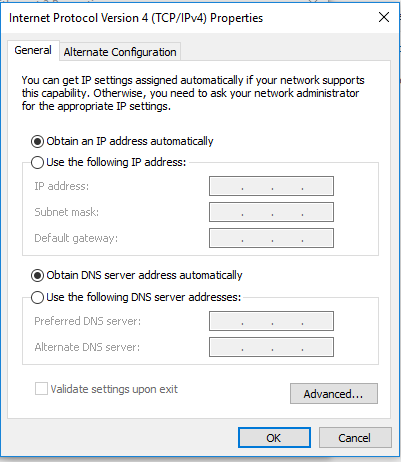
\includegraphics[scale=.8]{image4}
	\end{center}
	Cek IP Address dari komputer tersebut menggunakan aplikasi Comment Prompt dengan perintah ipconfig /all.
	\begin{center}
		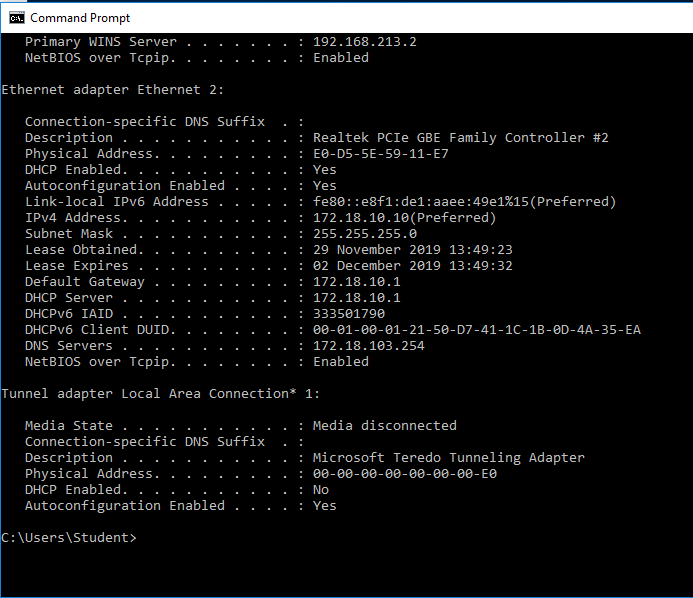
\includegraphics[scale=.4]{image5}
	\end{center}
	IP address yang didapat tidak bisa 172.18.10.100 , karena dhcp pool yang dikonfigurasi adalah 172.18.10.2 sampai 172.18.10.10
	\begin{center}
		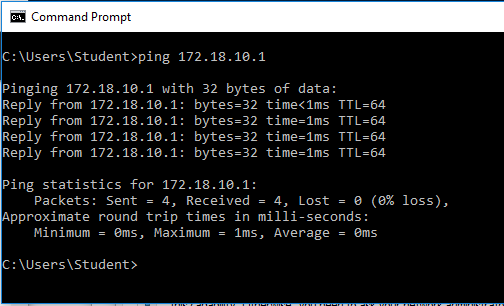
\includegraphics[scale=.7]{image6}
	\end{center}
	Lakukan tes koneksi dengan perintah Ping ke Gateway-nya: 172.18.10.1 dan pastikan terkoneksi.
	
	\item \textbf{Cek Koneksi ke Internet Melalui Router Menggunakan Terminal.}\\
	\begin{center}
		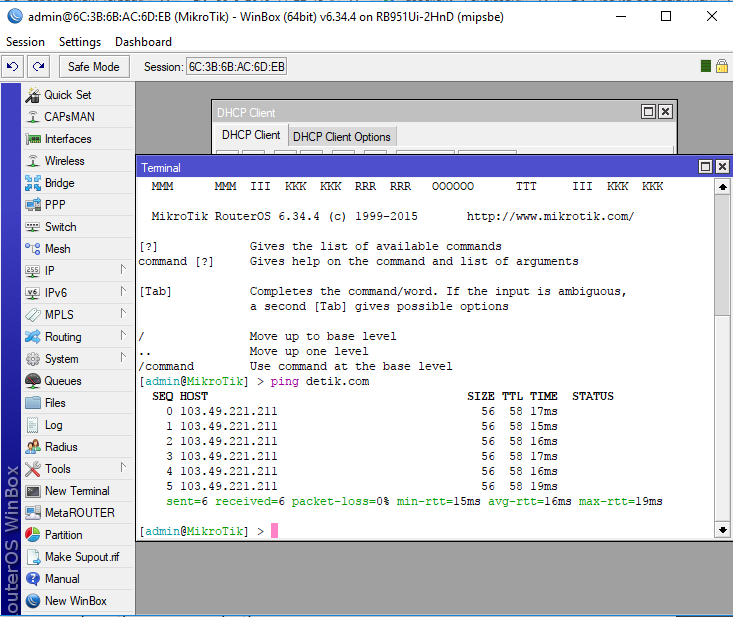
\includegraphics[scale=.6]{Capture11}
	\end{center}
	Klik New Terminal, akan muncul kotak window Terminal, berikan perintah untuk cek koneksi ke situs berita: www,detik.com koneksi dengan perintah Ping dan pastikan terkoneksi.
	
	\item \textbf{Cek Koneksi ke Internet Melalui PC yang terhubung ke Ether2 maupun Ether2.}
	Jalankan aplikasi Command Prompt, berikan perintah untuk cek koneksi ke situs berita: www,detik.com koneksi dengan perintah Ping dan hasilnya sama seperti pada gambar berikut yang berarti tidak terkoneksi.
	\begin{center}
		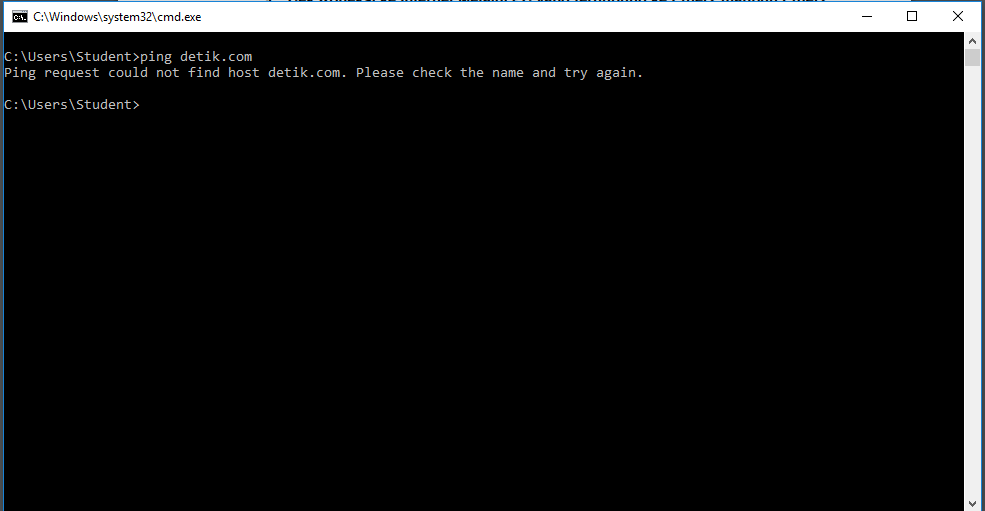
\includegraphics[scale=.5]{Capture12}
	\end{center}
	
	\item \textbf{Setting Source-Network Address Translation (Src-NAT),}\\
	Cek koneksi pada praktik ke-10 membuktikan bahwa router sudah terkoneksi dengan jaringan internet, sedangkan pada praktik ke-11 membuktikan bahwa kedua PC yang terhubung ke Ether2 dan Ether3 belum terkoneksi dengan jaringan internet. Setting ini akan mengubah source address dari sebuah paket data, yang berasal dari PC yang terhubung ke Ether2 diubah ke source address-nya milik Ether1 yang sudah sudah terbukti dapat terkoneksi dengan internet, sehingga menjadikan PC yang terhubung ke Ether2 dapat terkoneksi dengan jaringan internet.
	
	Pilih menu IP → Firewall, akan muncul kotak window Firewall, lalu klik tab NAT.	
	Kemudian klik tombol + , 
	\begin{center}
		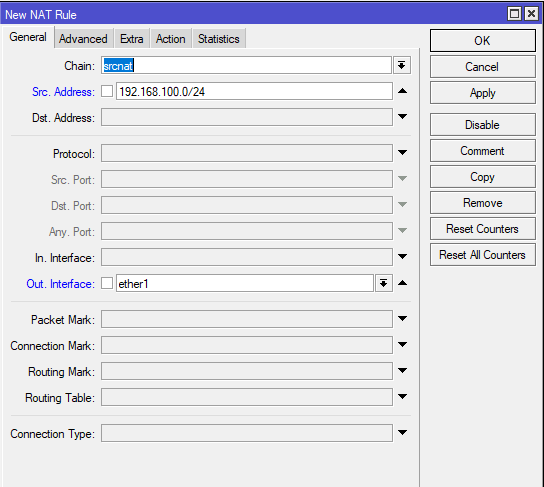
\includegraphics[scale=.8]{Capture13}
	\end{center}
	maka akan muncul kotak window New NAT Rule, klik tab General dan lakukan pengisian pada Chain: srcnat (untuk mengubah source address dari sebuah paket data), Src. Address: 192.168.100.0/24 (source address yang diubah memiliki alamat network 192.168.100.0 dan netmask: 255.255.255.0) dan Out. Interface:Ether1 (interface yang akan dikenali dari luar).	
	\begin{center}
		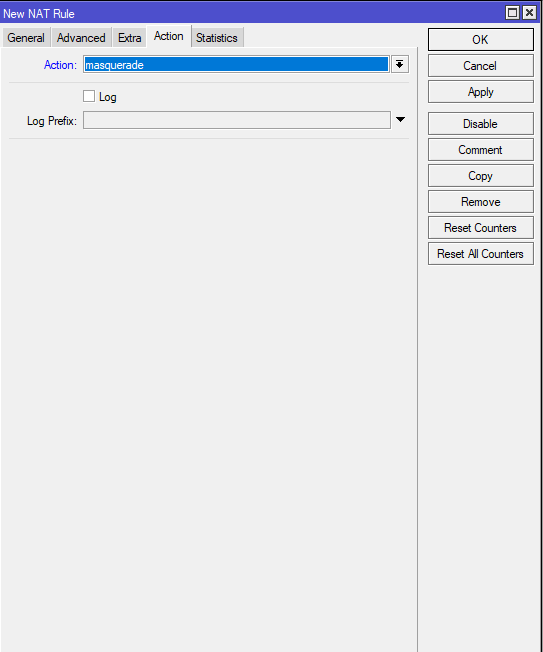
\includegraphics[scale=.5]{Capture14}
	\end{center}
	Klik tab Action, pada isian Action:masquerade (ini berarti bahwa source address 192.168.100.0/24 ditopengkan sehingga nanti akan dikenal dengan source addres-nya Ether1, yaitu: 172.17.25.106/24, kemudian klik tombol Apply.
Kemudian klik tombol OK, yang berarti setting Src-NAT telah selesai.
	\begin{center}
		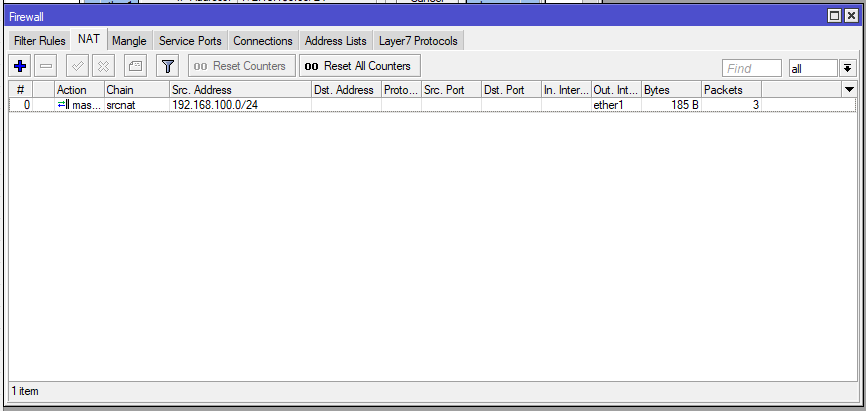
\includegraphics[scale=.5]{Capture15}
	\end{center}
	
	\item \textbf{Cek Kembali Koneksi ke Internet Melalui PC yang terhubung ke Ether2 maupun Ether2.}\\
	Jalankan aplikasi Command Prompt, berikan perintah untuk cek koneksi ke situs berita: www.detik.com koneksi dengan perintah Ping dan hasilnya akan berbeda seperti pada gambar berikut.
\\
	
	Pada PC yang terhubung ke Ether2.
	\begin{center}
		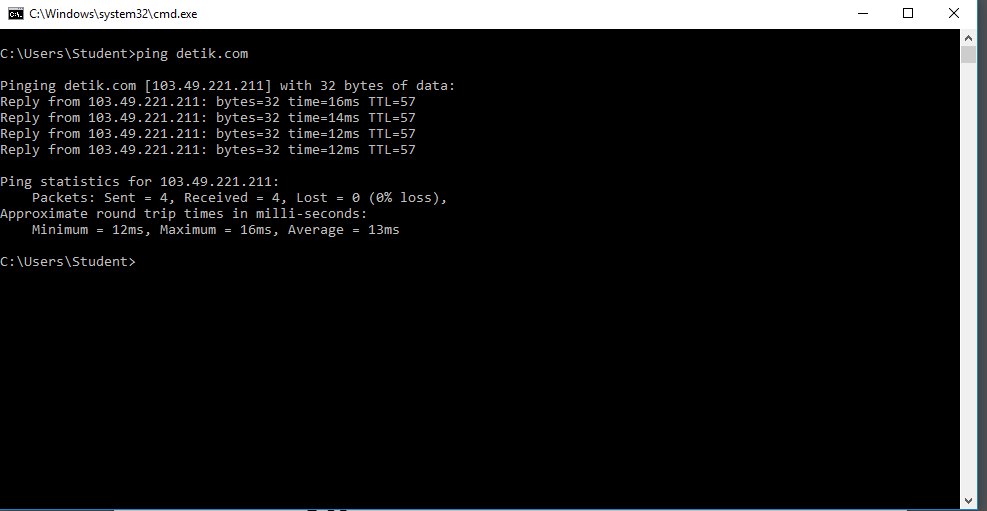
\includegraphics[scale=.4]{Capture16}
	\end{center}
\end{enumerate}

\section{Latihan}
Pilih menu IP → Firewall, akan muncul kotak window Firewall, lalu klik tab NAT.	
Kemudian klik tombol + , 
\begin{center}
	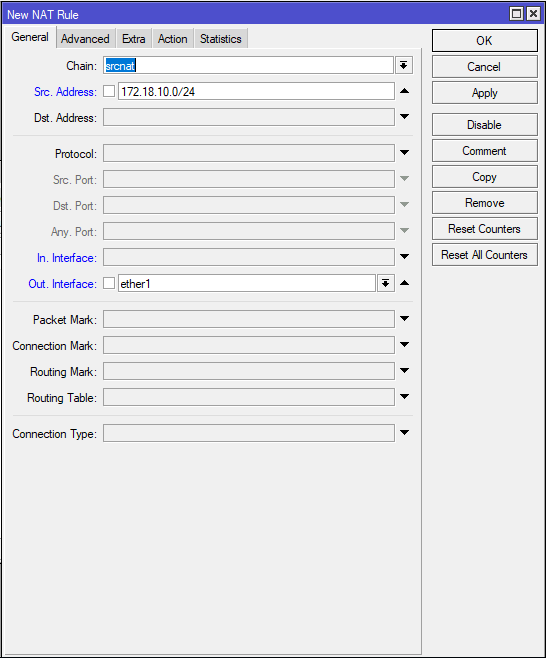
\includegraphics[scale=.5]{lat1}
\end{center}
maka akan muncul kotak window New NAT Rule, klik tab General dan lakukan pengisian pada Chain: srcnat (untuk mengubah source address dari sebuah paket data), Src. Address: 172.18.10.0/24 (source address yang diubah memiliki alamat network 172.18.10.0 dan netmask: 255.255.255.0) dan Out. Interface:Ether1 (interface yang akan dikenali dari luar).	
\begin{center}
	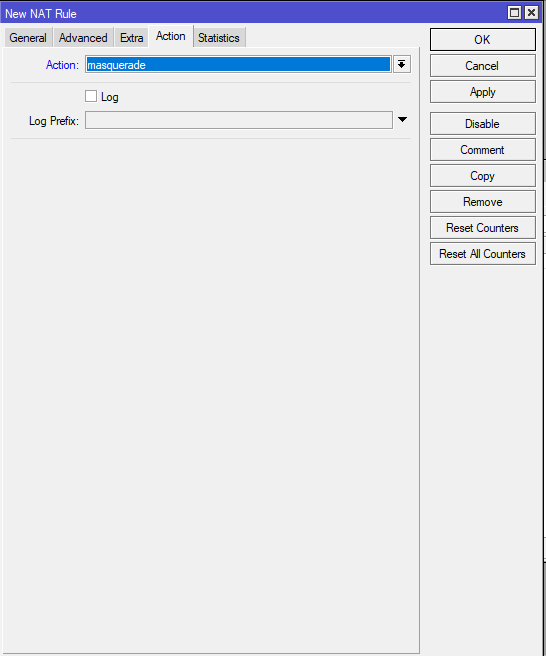
\includegraphics[scale=.5]{lat2}
\end{center}
Klik tab Action, pada isian Action:masquerade (ini berarti bahwa source address 172.18.10.0/24 ditopengkan sehingga nanti akan dikenal dengan source addres-nya Ether1, yaitu: 172.17.25.106/24, kemudian klik tombol Apply.
Kemudian klik tombol OK, yang berarti setting Src-NAT telah selesai.
\begin{center}
	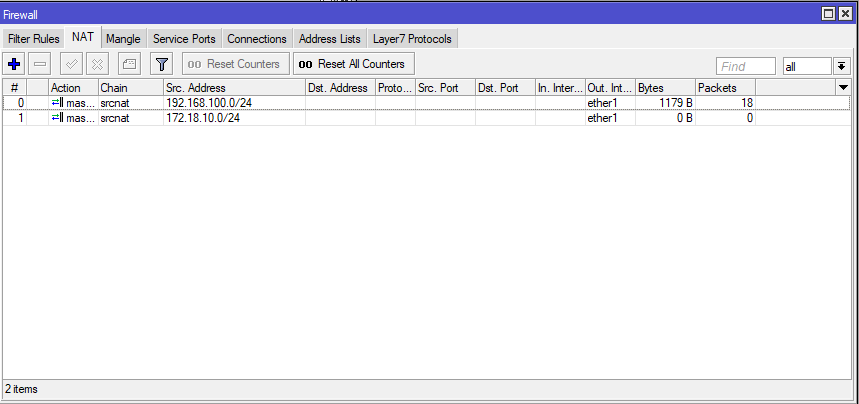
\includegraphics[scale=.5]{lat3}
\end{center}

\section{Tugas}
\begin{enumerate}
	\item Hasil cek koneksi pada praktik ke-13 berbeda, antara cek koneksi internet pada PC yang terhubung ke Ether2 dengan yang terhubung ke Ether3 karena yang dikonfigurasi untuk dimask adalah jaringan hanya 192.168.100.0
	
	\item Perbedaan Out. Interface dengan In. Interface adalah Out adalah interface yang menjadi tujuan dari paket jaringan, sedangkan in adalah darimana paket jaringan berasal. 
\end{enumerate}

\newpage
\section{Kesimpulan}
Setelah praktik ini mahasiswa mampu melakukan konfigurasi NAT pada mikrotik untuk mengakses Internet
\end{document}